\documentclass[a4paper]{article}

%%%%%%%%%%%%%%%%%%%%%%%%%%%%%%%%%%%%%%%%%%%%%%
% Gestion du français et des accents %
\usepackage[utf8x]{inputenc}
\usepackage[T1]{fontenc}
\usepackage[greek, french]{babel}
%%%%%%%%%%%%%%%%%%%%%%%%%%%%%%%%%%%%%%%%%%%%%%

%%%%%%%%%%%%%%%%%%%%%%%%%%%%%%%%%%%%%%%%%%%%%%
% Gestion des Sections et de la Table des matières %
\setcounter{secnumdepth}{3}
\setcounter{tocdepth}{3}

\usepackage[]{titletoc}
%\titlecontents
%		{section}
%		[left]
%		{au-dessus}
%		{avant (si label)}
%		{avant (sans label)}
%		{remplissage et n°page}
%		[après]



%%%   Section   %%%

\titlecontents
	{section}
	[25pt]
	{\addvspace{0.75pc}}
	{\normalfont\scshape\contentslabel{25pt}}
	{}
	{\normalsize\hfill\bfseries ~\thecontentspage\vspace{-3pt}\hrule}
	[\addvspace{0.5pc}]
	


%%%   Sous-Section   %%%

\titlecontents
	{subsection}
	[75pt]
	{\addvspace{-0.5pc}}
	{\normalfont\small\contentslabel{30pt}}
	{}
	{\normalsize\dotfill\small\thecontentspage}
	[]



%%%   Sous-sous-Section   %%%

\titlecontents
	{subsubsection}
	[125pt]
	{\addvspace{-0.5pc}}
	{\normalfont\footnotesize\contentslabel{30pt}\itshape}
	{}
	{\normalsize\hfill\footnotesize\itshape\thecontentspage}
	[]
	
\contentsfinish
%%%%%%%%%%%%%%%%%%%%%%%%%%%%%%%%%%%%%%%%%%%%%%

%%%%%%%%%%%%%%%%%%%%%%%%%%%%%%%%%%%%%%%%%%%%%%
% Gestion des marges du document %

\usepackage{geometry}

\geometry{
paperwidth=21cm,
%width=15.5cm,
left=3cm,
right=3cm,
paperheight=29.7cm,
%height=26.5cm,
top=3cm,
bottom=3cm,
headheight=0cm,
headsep=0cm,
footskip=1cm
}
%%%%%%%%%%%%%%%%%%%%%%%%%%%%%%%%%%%%%%%%%%%%%%

\usepackage{graphicx}
\usepackage{setspace}
\usepackage{mathtools}
\usepackage{rotating}
\usepackage{multirow}

%\usepackage[mathletters]{ucs}

\DeclareFontEncoding{LS1}{}{}
\DeclareFontSubstitution{LS1}{stix}{m}{n}
\DeclareSymbolFont{symbols4}{LS1}{stixbb}{m}{it}
\DeclareMathSymbol{\varhexagonblack}{\mathord}{symbols4}{"DD}
\DeclareMathSymbol{\hexagonblack}   {\mathord}{symbols4}{"DE}


\usepackage{setspace}
\usepackage{amssymb}
\usepackage{numprint}

\def\nbR{\ensuremath{\mathrm{I\! R}}}


\renewcommand{\thesection}{\Roman{section}}
\renewcommand{\thesubsubsection}{\roman{subsubsection}}

\usepackage{xlop}
\usepackage{ulem}

\parindent=1cm

\usepackage[bottom]{footmisc}
\usepackage[dvipsnames]{xcolor}

\usepackage{footnote}
\makesavenoteenv{tabular}





\begin{document}

	\begin{titlepage}
		\begin{center}
		
			\Huge	 \textbf{Mathématiques}\\
			\bigskip \smallskip
		
			\Large	 \textbf{$\varhexagonblack$ Section 3 - Trigonométrie $\varhexagonblack$}\\
			\bigskip
		
			\large	 Clément \sc{Campana}  \\ 
			\smallskip
		
			\normalfont	Juillet 2022\\
		
		\end{center}
		
		%\onehalfspacing
		\doublespacing
		\tableofcontents
		\singlespacing

	\end{titlepage}




% -------------------------------------------------------------

	\section{Premier pas en Trigonométrie}

		La Trigonométrie est, comme son nom l'indique, une discipline mathématique qui a comme objectif de "mesurer" les triangles.

		Plus clairement, son but est de pouvoir déduire l'ensemble des informations disponibles dans un 
		triangle à partir du minimum d'information sur ce triangle.
		Comme vu dans la Section 2, un triangle est un polygone à 3 côtés, 
		et la somme des 3 angles d'un triangle vaut 180°, $\pi$ rad ou 200 gr.

		En général, en Trigonométrie, on se focalise principalement sur les \textit{triangles rectangles}, 
		puis on généralise les théorèmes que nous avons démontré à tous les triangles.

		\subsection{Construction d'un triangle}
	
			Les triangles ont une particularité les différenciant des autres polygones :

			\textbf{En connaissant la longueur de 3 côtés d'un triangle, il est possible de parfaitement construire ce triangle.}

			Dans les autres polygones, cette condition n'est pas suffisante pour le construire\footnote{
				Par exemple, si l'on prend un quadrilatère donné, 
				où l'on a fixé la longueur de 4 côtés,
				il est possible de "l'écraser" afin d'obtenir un autre
				quadrilatère ayant les mêmes longueurs de côtés.
				En revanche, les angles formés par les côtés de ce quadrilatère 
				ne seront pas les mêmes que ceux du quadrilatère de départ.
				
				Ainsi, à partir d'un losange, il est possible de créer un carré, 
				en fonction des angles choisis entre les côtés.

				Pour la même raison, 
				les polygones ayant plus de côtés ne sont pas constructibles
				en connaissant uniquement les longueurs de leurs côtés.
			}.

			\medbreak

			Pour tracer un triangle à l'aide de \textit{trois longueurs}, 
			il faut tracer un segment mesurant une des trois longueurs choisies, 
			puis tracer deux cercle ayant comme centre les extrémités du segment 
			et comme rayons les deux autres longueurs voulues pour le triangle. 
			Les cercles se croisent en deux points, 
			avec lesquelles ont peut construire deux triangles symétriques.

			\medbreak

			Mais l'on peut aussi remplacer un des cercles ou les deux 
			cercles par une ou des demi-droites, 
			ayant un angle interne d'une valeur choisie. 
			Cette demi-droite et le cercle ou ces deux demi-droites 
			vont se croiser en un point, le troisième sommet du triangle.

			Voici un tableau récapitulatif des différentes possibilités de construction d'un triangle, 
			en fonction du nombre d'informations connues sur celui-ci :

			\begin{center}
					\renewcommand{\arraystretch}{1.25}
					\begin{tabular}{|c|c|c|c|c|}
						\hline
									           & \textbf{Aucune longueur}         & \textbf{1 longueur}              & \textbf{2 longueurs}             & \textbf{3 longueurs}             \\
						\hline
						\textbf{Aucun angle}   & \textcolor{Red}{Inconstructible} & \textcolor{Red}{Inconstructible} & \textcolor{Red}{Inconstructible} & \textcolor{Green}{Constructible} \\
						\hline
						\textbf{1 angle}       & \textcolor{Red}{Inconstructible} & \textcolor{Red}{Inconstructible} & \textcolor{Green}{Constructible} & \textcolor{Green}{Constructible} \\
						\hline
						\textbf{2 ou 3 angles}\footnote[2]{
							En connaissant deux angles d'un triangle, 
							il est possible de déduire le troisième, 
							car la somme des trois angles d'un triangle 
							correspond à un angle plat.
											} & Triangles semblables\footnote[3]{
											Avec deux ou trois angles, 
											il n'est pas possible de construire un triangle en particulier,
											mais seulement une collection de triangles semblables entre-eux.
										}& \textcolor{Green}{Constructible} & \textcolor{Green}{Constructible} & \textcolor{Green}{Constructible} \\
						\hline
					\end{tabular}
			\end{center}

			Nous pouvons en conclure qu'un triangle en particulier, 
			est traçable à l'aide d'une longueur et de deux autres mesures 
			(des angles ou des longueurs).

			\begin{center}
				\makebox[\textwidth][c]{
					\begin{tabular}{cc}
						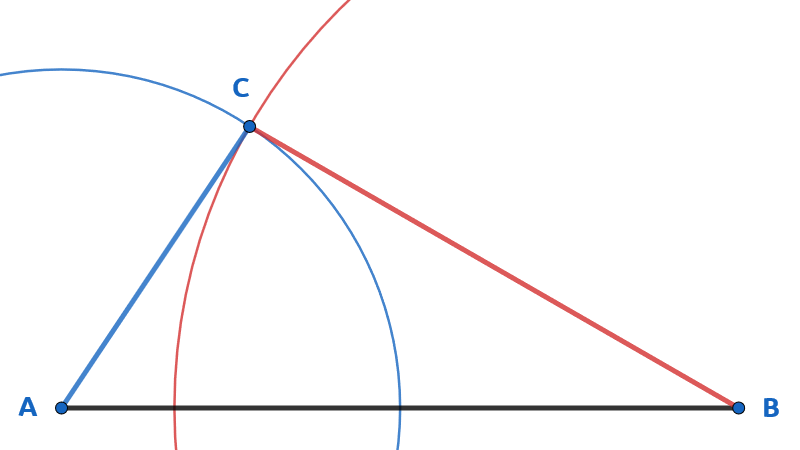
\includegraphics[width=7cm]{Image/Triangle/Triangle_construction_3_longueurs.png}         &
						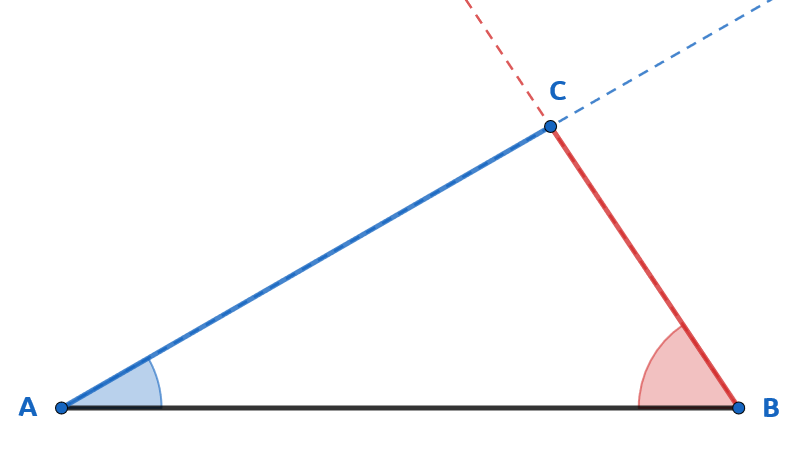
\includegraphics[width=7cm]{Image/Triangle/Triangle_construction_1_longueur_2_angles.png} \\

						\textit{Triangle construit avec 3 longueurs} & \textit{Triangle construit avec 1 longueur et 2 angles} \\
					\end{tabular}
				}
			\end{center}

			Cette propriété unique aux triangles, nous sera très utile par la suite.

			\medbreak


\newpage
		
		\subsection{Fonctions trigonométriques}

		\subsubsection{Relation entre les longueurs des côtés d'un triangle rectangle}

			Prenons un triangle rectangle, 
			dont (par définition) nous connaissons un des angles, 
			son angle droit (qui vaut 90°, $\frac{\pi}{2}$ rad ou 100 gr).

			Prenons un autre de ces angles, que nous appellerons $\alpha$. 
			
			Nous connaissons ainsi deux angle, l'angle droit et l'angle $\alpha$.
			Comme nous savons que la somme des trois angles du triangle vaut un angle plat,
			nous pouvons déduire la mesure du dernier angle.
			Notre troisième angle (que nous nommerons $\beta$) vaut en degré : $\beta = 180^\circ - (90^\circ + \alpha) = 90^\circ - \alpha$

			\medbreak

			Maintenant, nous avons obtenues les mesures des trois angles du triangle.
			Comme vu plus précédemment dans le tableau,
			avec uniquement 3 angles, il est possible de construire une collection de \textbf{triangles tous semblables entre-eux}.

			Afin d'être plus clair, nommons les côtés de notre triangle $a$, $b$ et $c$, en fonction de leur taille.
			Le côté $a$ sera le plus court, le côté intermédiaire sera le $b$ et le plus long sera le $c$.

			\medbreak

			Prenons deux de triangles de cette collection, le triangle 1 et le triangle 2. 
			Leurs côtés mesures $a_1$, $b_1$, $c_1$ et $a_2$, $b_2$, $c_2$.
			Comme ces triangles sont semblables, 
			leurs côtés sont proportionnels entre-eux,
			ce qui signifie que $\frac{a_1}{a_2} = \frac{b_1}{b_2} = \frac{c_1}{c_2}$.

			Cette propriété implique que, les rapports entre les côtés dans un triangle 
			vont être égaux à ceux des mêmes côtés dans un autre triangle semblable au premier.

			\medbreak

			Mathématiquement, cela signifie que, 
			pour les côtés $a$ et $b$ de deux triangles semblables, 
			on a $\frac{a_1}{b_1} = \frac{a_2}{b_2}$.

			Démontrons cette propriété :
			$\frac{a_1}{a_2} = \frac{b_1}{b_2}$
			$\Longleftrightarrow a_1 \times b_2 = a_2 \times b_1$
			$\Longleftrightarrow \frac{a_1 \times b_2}{b_1} = a_2$
			$\Longleftrightarrow \frac{a_1}{b_1} = \frac{a_2}{b_2}$

			Les démonstrations des relations entre les autres côtés sont analogues.

			\medbreak

			Cela signifie que les \textbf{rapports entre les longueurs} des côtés dans triangle, ne dépend que des mesures des angles.

			De plus, comme nous sommes dans un triangle rectangle,
			tous les angles du triangle sont soit fixé à l'avance (l'angle droit), 
			ou ne dépendent que de la mesure de l'angle $\alpha$. 

			\medbreak

			Et enfin, 
			nous pouvons en conclure que les rapports entre tous les côtés d'un triangle rectangle,
			ne dépendent que de la mesure de l'angle $\alpha$.

			\bigbreak
			\bigbreak

		\subsubsection{Définition des fonctions trigonométriques élémentaires}

			Comme montré plus tôt, les rapports en chaque côté d'un triangle rectangle, 
			ne dépendent que de l'angle $\alpha$ (défini comme étant un autre angle que l'angle droit).
			
			En revanche, ce rapport entre longueurs n'est pas simplement constant, 
			il varie de manière complexe en fonction de l'angle $\alpha$.
			
			\medbreak

			Pour prendre en compte ces variations, et donc pouvoir obtenir une relation chiffrée, 
			les mathématiciens ont construits un grand arsenal de fonctions trigonométriques\footnote{
				Une grande partie des fonctions trigonométriques créées sont rarement utiles, 
				pour en savoir plus sur ces fonctions délaissées, rendez-vous en Annexe, à la page \pageref{fonction_trigo_chelous}.
			}. 
			

			{\noindent Les fonctions trigonométriques les plus utiles sont : }
			
			\begin{itemize}
				\item [•] La fonction \emph{sinus}, notée $\sin$.
				\item [•] La fonction \emph{cosinus}, notée $\cos$.
				\item [•] La fonction \emph{tangente}, notée $\tan$.
			\end{itemize}

			\bigskip

			{\noindent Dans ces relations, on utilise : }
			
			\begin{itemize}
				\item [•] L'angle $\alpha$, définit précédemment.
				\item [•] La cathète opposée à l'angle $\alpha$ (noté $O$ et généralement appelée "côté opposé").
				\item [•] La cathète adjacente à l'angle $\alpha$ (noté $A$ et généralement appelée "côté adjacent").
				\item [•] L'hypoténuse du triangle (noté $H$).
			\end{itemize}

\newpage

			Voici les relations en questions, qui sont les définitions respectives de la fonction sinus, cosinus et tangente :
			
			\begin{center}
				
				\renewcommand{\arraystretch}{2}
				\begin{tabular}{|c|ccc|}
					\hline
					\textbf{Fonction} & \textbf{Définition}                                                                 & \multicolumn{2}{c|}{\textbf{Résumé}} \\
					\hline
					\textbf{Sinus}    & $\sin(\alpha) =$ {\Large $\frac{\text{Cathète Opposée}}{\text{Hypoténuse}}$       } & $\sin(\alpha) = \frac{\text{O}}{\text{H}} \Longrightarrow \text{S = O / H} $ & \textit{SOH} \\
					\textbf{Cosinus}  & $\cos(\alpha) =$ {\Large $\frac{\text{Cathète Adjacente}}{\text{Hypoténuse}}$     } & $\cos(\alpha) = \frac{\text{A}}{\text{H}} \Longrightarrow \text{C = A / H} $ & \textit{CAH} \\
					\textbf{Tangente} & $\tan(\alpha) =$ {\Large $\frac{\text{Cathète Opposée}}{\text{Cathète Adjacente}}$} & $\tan(\alpha) = \frac{\text{O}}{\text{A}} \Longrightarrow \text{T = O / A} $ & \textit{TOA} \\
					\hline
				\end{tabular}
			\end{center}

			Un bon moyen mnémotechnique pour retenir ces définitions, 
			est l'expression "\textit{Casse-toi !}". 
			On peut l'obtenir en utilisant les résumés des définitions à droite, 
			réarrangeant les définitions, en mettant celle du cosinus en premier.
			Ainsi, on obtient "\textit{CAH, SOH, TOA}".
			
			\medbreak

			A l'aide de ces relations, 
			il est possible de connaître toutes les longueurs de 
			tous les côtés d'un triangle rectangle à l'aide uniquement 
			de la mesure d'un de ses angles et d'une longueur d'un des côtés.

			
			\noindent {
				\makebox[\textwidth][c]{
					\renewcommand{\arraystretch}{1.75}
					\begin{tabular}{lc|c|c|cc}
						\multicolumn{5}{l}{Exemple :} & \multirow{3}{*}{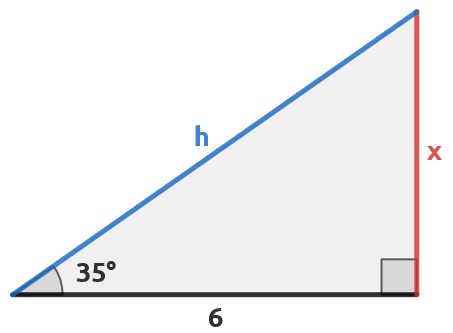
\includegraphics[width=3.1cm]{Image/Triangle/Triangle_sinus_cosinus.png}} \\
						
						\phantom{Exempl} & \textit{CAH} & $\text{C = A / H}$ & $\cos(35^\circ) = \frac{6}{h}$ & $h = \frac{6}{\cos(35^\circ)} \approx 7,32 $ & \\
						                    & \textit{TOA} & $\text{T = O / A}$ & $\tan(35^\circ) = \frac{x}{6}$ & $x = 6 \times \tan(35^\circ) \approx 4,20 $ &\\
					\end{tabular}
				}
			}

			\bigbreak
			\bigbreak
			\bigbreak
			\bigbreak
			\bigbreak
			\bigbreak



		\subsubsection{Lien entre ces trois fonctions}

			De plus,
			il est possible d'établir un lien entre ces trois fonctions :
			{ \LARGE $$ \tan(\alpha) = \frac{\sin(\alpha)}{\cos(\alpha)} $$}

			\medbreak
			\medbreak

			Pour démontrer cette relation, 
			on peut utiliser la définition de la tangente, 
			puis remplacer les longueurs des côtés à l'aide 
			des définitions des fonctions sinus et cosinus :

			\medbreak

			\begin{itemize}
				\item [ ] $\text{Cathète Opposée}   = \sin(\alpha) \times \text{Hypoténuse}$
				\item [ ] $\text{Cathète Adjacente} = \cos(\alpha) \times \text{Hypoténuse}$
			\end{itemize}

			\bigbreak

			\begin{Large}
			\begin{itemize}
				\item [ ] $\tan(\alpha) = \frac{\text{Cathète Opposée}}{\text{Cathète Adjacente}} = \frac{\sin(\alpha) \times \text{Hypoténuse}}{\cos(\alpha) \times \text{Hypoténuse}} = \frac{\sin(\alpha)}{\cos(\alpha)}$
			\end{itemize}
			\end{Large}

\newpage

	\section{Cercle trigonométrique}

		\subsection{Unité d'angle reine en Trigonométrie : le radian}

			Comme présenté dans la Section 2, 
			il existe plusieurs unités d'angle différentes.

			L'unité la plus utilisée est le degré, 
			mais cette dernière n'est pas la plus adaptée 
			en mathématique, en particulier en Trigonométrie,
			où l'on préfère utiliser le radian.

			\medbreak

			Pour en savoir plus sur les définitions des unités d'angle,
			rendez-vous dans la Section 2, dans la partie consacrée aux Angles.

			\subsubsection*{Rappel de la définition du radian}

				Pour un angle donné, 
				la mesure en radians de cet angle est égale 
				à la longueur de l'arc de cercle intercepté par cet angle,
				sur un cercle de rayon 1.

				Ainsi, le radian est l'unité étant la plus cohérente mathématiquement,
				car elle est basée sur la longueur de l'arc de cercle formé.
				Cette cohérence a donné à cette unité un statut privilégié\footnote{
					Au premier abord, 
					le statut privilégié du radian ne semble pas solidement justifiée.
					C'est à dire que, mis à part la \textit{beauté mathématique} 
					de la définition du radian par rapport au degré, 
					pourquoi cette unité est a préféré à une autre ?

					Cette préférence provient de certaines propriétés mathématiques 
					qui ne sont vrai que si l'unité d'angle est le radian.
					En particulier, lorsque l'on dérive ou intègre une 
					fonction trigonométrique ou encore lorsque 
					l'on utilise un développement limité de 
					cette fonction trigonométrique.

					Dans ces cas, l'angle peut se retrouver en facteur, 
					position où seule la mesure en radians d'un angle a un sens.
				} en mathématique, en particulier en Trigonométrie.


				Cependant, le périmètre d'un cercle étant égal à $2 \pi$, 
				on retrouve la constante $\pi$ un peu partout 
				dans les mesures d'angles usuels. 
				Cette constante rend l'utilisation 
				de cette constante peu intuitive, 
				ce qui explique certainement pourquoi cette unité, 
				mathématiquement meilleure que le degré, 
				ne s'est pas imposée au plus grand nombre 
				comme remplaçante de cette vielle unité.

			
		\subsection{Cercle trigonométrique}

			En mathématique (et en science plus globalement), l'unité reine est le radian, c'est donc cette dernière que nous allons utiliser ici, à partir de maintenant.

			Pour représenter des angles et bien comprendre leur lien avec les fonctions trigonométriques, on utilise généralement le cercle trigonométrique. Ce cercle est centré autour de l'origine du repère et à un rayon égal à 1, ce cercle est représenté ci-dessous. 

			XXXXXXXXXXXXXXXXXXXXXXXXXXXXXXXXXXXXXXXXXXXXXXXXXXXXXXXXXXXXXXXXX

			Un angle représenté sur ce cercle est “orienté”, c'est-à-dire qu'il commence et qu'il termine aux extrémités le définissant.

			L'axe de départ de tous les angles représentables sur le cercle est l'axe des abscisses (plus précisément, l'axe des abscisses positives). L'angle est mesuré entre deux demi-droites, celui des abscisses positives et une autre servant à terminer l'angle, ces deux demi-droites partent de l'origine du repère.

			L'orientation des angles correspond au sens indiqué par la flèche en haut à droite du cercle, ce sens, inverse au sens horaire (celui dans lequel tournent les aiguilles d'une montre), est appelé sens trigonométrique (ou sans antihoraire).

			Cette orientation donne un signe aux angles, ainsi les angles $\alpha$ et $\beta$ sont des angles positif et les angles $\gamma$ et $\theta$ sont négatifs. En tournant autour du cercle, on retrouve ainsi n'importe quelle angle possible. 

		\subsection{Lien avec les fonctions trigonométriques}

			Sur le cercle trigonométrique, il est possible de retrouver simplement le sinus et le cosinus d'un angle représenté sur le cercle. Appelons cet angle $\theta$. En effet, en projetant le point A (celui étant à l'intersection entre le cercle et la demi-droite terminant l'angle étudié) sur l'axe des abscisses, alors on forme le point $X_A$, et à l'aide des calculs vus précédemment, on trouve que la longueur du segment [O$X_A$] est égal à $\cos(\theta)$. En effet, le triangle OA$X_A$ est un triangle rectangle, il est donc possible d'utiliser la formule définissant le cosinus, soit :

			$\cos(\theta) = \frac{\text{Cathète Adjacente}}{\text{Hypoténuse}} = \frac{\text{A}}{\text{H}}$

			Dans notre cas, on a donc :

			$\cos(\theta) = \frac{\text{O}X_A}{\text{OA}} = \frac{\text{O}X_A}{1}$

			Ainsi $\text{O}X_A = \cos(\theta)$

			Il est également possible de projeter le point A sur l'axe des ordonnées, pour former le point $Y_A$. Et de manière analogue, on démontre aisément que $\text{O}Y_A = \sin(\theta)$.

			J'ai trouvé un moyen mnémotechnique pour retenir quel axe est celui où l'on retrouve le sinus de l'angle. L'abréviation de sinus c'est sin, ce qui correspond au début du mot “singe”, les singes montent dans les arbres, alors l'axe des sinus est l'axe verticale de notre repère.

			De plus, on peut aussi retrouver graphiquement la tangente, pour un angle $\theta$, c'est la longueur du segment perpendiculaire à la droite (OA) tangente (géométrique) au cercle trigonométrique qui intercepte l'axe des abscisses.

		\subsection{Arithmétique modulaire}

			L'arithmétique modulaire est une branche de l'arithmétique étudiant le reste dans la division euclidienne d'un nombre, en fonction d'un autre, qu'on appellera module. 

			L'etude se fait uniquement sur les restes de cette division euclidienne, ainsi les valeurs étudiées pouvant 

		\subsection{Mesure principale}

	\section{Propriété des fonctions sin / cos / tan}

		\subsection{Valeurs remarquables}

			Annexe autres valeurs remarquables 

		\subsection{Propriétés de ces fonctions}

		\subsection{Représentation graphique}

		\subsection{Étude de fonction (Variation, …)}

	\section{Fonctions inverses arcsin / arccos / arctan}

		\subsection{Propriétés de ces fonctions}

		\subsection{Représentation graphique}

	\section{Formules trigonométriques}

		normalesup.org/~dconduche/prepas/PT/cours/ChapitreFicheTrigo.pdf)

	\section{Lecture de la table}

	\section{Annexe}

		\subsection*{Fonctions trigonométriques chelous} \label{fonction_trigo_chelous}

		Fonctions trigonométriques chelous selon Github copilot :

		\begin{itemize}
				\item [•] La fonction sinus, notée $\sin$.
				\item [•] La fonction cosinus, notée $\cos$.
				\item [•] La fonction tangente, notée $\tan$.
				\item [•] La fonction cotangente, notée $\cot$.
				\item [•] La fonction sécante, notée $\sec$.
				\item [•] La fonction cosécante, notée $\csc$.
				\item [•] La fonction exsecante, notée $\text{exsec}$.
				\item [•] La fonction excosécante, notée $\text{excsc}$.
				\item [•] La fonction versine, notée $\text{vers}$.
				\item [•] La fonction coversine, notée $\text{covers}$.
				\item [•] La fonction haversine, notée $\text{havers}$.
				\item [•] La fonction hacoversine, notée $\text{hacovers}$.
				\item [•] La fonction exverse, notée $\text{exvers}$.
				\item [•] La fonction excovers, notée $\text{excovers}$.
				\item [•] La fonction vercosine, notée $\text{vercos}$.
				\item [•] La fonction coverscosine, notée $\text{coverscos}$.
				\item [•] La fonction havercosine, notée $\text{havercos}$.
				\item [•] La fonction hacoverscosine, notée $\text{hacoverscos}$.
				\item [•] La fonction exvercosine, notée $\text{exvercos}$.
				\item [•] La fonction excoverscosine, notée $\text{excoverscos}$.
				\item [•] La fonction exsecant, notée $\text{exsec}$.
				\item [•] La fonction excosecant, notée $\text{excsc}$.
				\item [•] La fonction exsecant, notée $\text{exsec}$.
			\end{itemize}





\end{document}